\documentclass{article}
\usepackage{graphicx}
\usepackage{url}
\usepackage{tikz}
\usepackage{caption}
\usepackage{listings}



\title{Final Project cw}
\author{Kian Sharifan}
\date{January 2025}

\begin{document}

\maketitle
\newpage
\tableofcontents
\newpage

\section{Git and GitHub}
\subsection{Repository Initialization and Commits}
\begin{enumerate}
    \item first you make the repository
    \item you clone the repository on your pc
    \item you make the main.tex file
\end{enumerate}
\subsection{GitHub Actions for LaTeX Compilation}
\begin{enumerate}
    \item first you make the directory and the main.yml file
    \item then you give the permissions to the repository
    \item a very big challenge for me was the giving permissions to it
\end{enumerate}

\section{Exploration Tasks}
\subsection{Vim Advanced Features}
\begin{enumerate}
    \item \textbf{Macros}:
    Macros in Vim allow you to record a sequence of keystrokes and then replay them at will. This is particularly useful for repetitive tasks.
    \item \textbf{Vim Scripting (VimL)}:
    Vim has its own scripting language, VimL, which allows you to write custom functions, automate tasks, and extend Vim’s functionality. This feature is useful for creating complex workflows or plugins.
    \item \textbf{Text Objects and Operator-Pending Mode}:
    Text objects allow you to operate on logical pieces of text, like words, sentences, or paragraphs. This makes editing faster and more intuitive.
\end{enumerate}
\subsection{Memory profiling}
\subsubsection{Memory Leak}
A memory leak occurs when a program allocates memory but fails to release it back after it’s no longer needed. Over time, these unreleased memory allocations accumulate, which can eventually cause the program to run out of memory, leading to degraded performance or crashes.\newline
\textbf{How Memory Leaks Happen:}
\begin{enumerate}
    \item Failing to Free Memory
    \item Lost References
    \item Improper Error Handling
\end{enumerate}
\newpage
\subsubsection{Memory profilers}
\textbf{Its purposes}:\newline
1.	Memory Leak Detection:
Valgrind helps identify memory that has been allocated but not properly freed, showing where and when the memory was allocated and where it wasn’t released. This is invaluable for tracking down memory leaks that can accumulate and cause performance degradation or program crashes.\newline\newline
	2.	Error Detection:
Valgrind detects issues such as use of uninitialized memory, accessing memory after it has been freed (use-after-free), and reading or writing out-of-bounds memory. These errors can lead to undefined behavior, crashes, or corruption of data.\newline\newline
	3.	Performance Profiling:
Valgrind also has tools like Cachegrind and Callgrind that allow you to analyze the performance of your program, helping you identify inefficient areas of code.\newline\newline
\textbf{How Valgrind Helps with Memory Leaks:}\newline
	•	Tracking Allocated Memory:
When running a program with Valgrind, it tracks every memory allocation (using functions like malloc, calloc, realloc, etc.) and deallocation (free). If any allocated memory is not freed before the program terminates, Valgrind reports it as a memory leak.\newline\newline
	•	Detailed Reports:
Valgrind provides detailed reports that show:\newline\newline
	•	The exact locations in the code where memory was allocated.\newline\newline
	•	The locations where memory was not freed.\newline\newline
	•	A summary of all memory leaks with the amount of memory lost and the stack trace to the allocation point.

\subsection{GNU/Linux Bash Scripting}
\subsubsection{fzf}
\begin{itemize}
    \item Fuzzy searching finds text matches that are close to a search term, even with typos or variations.
    \item ls: Lists the files and directories in the current directory.\newline|: The pipe (|) passes the output of ls (the list of files) to the next command.\newline fzf: Launches the fuzzy finder (fzf), which allows you to interactively search and select from the list of files.
\end{itemize}
\newpage
\subsubsection{Using fzf to find your favorite PDF}
\begin{enumerate}
    \item you use this command: fd -e pdf
    \item To select a .pdf file from the list using fzf, you can combine the fd command (for listing .pdf files) with fzf like this: fd -e pdf | fzf
\end{enumerate}
\subsubsection{Opening the file using Zathura}
you can use : zathura \$ (fd -e pdf | fzf) for that propose

\section{Git and FOSS}
\subsection{README.md}
\subsection{Issues}
\begin{figure}[h]
    \centering
    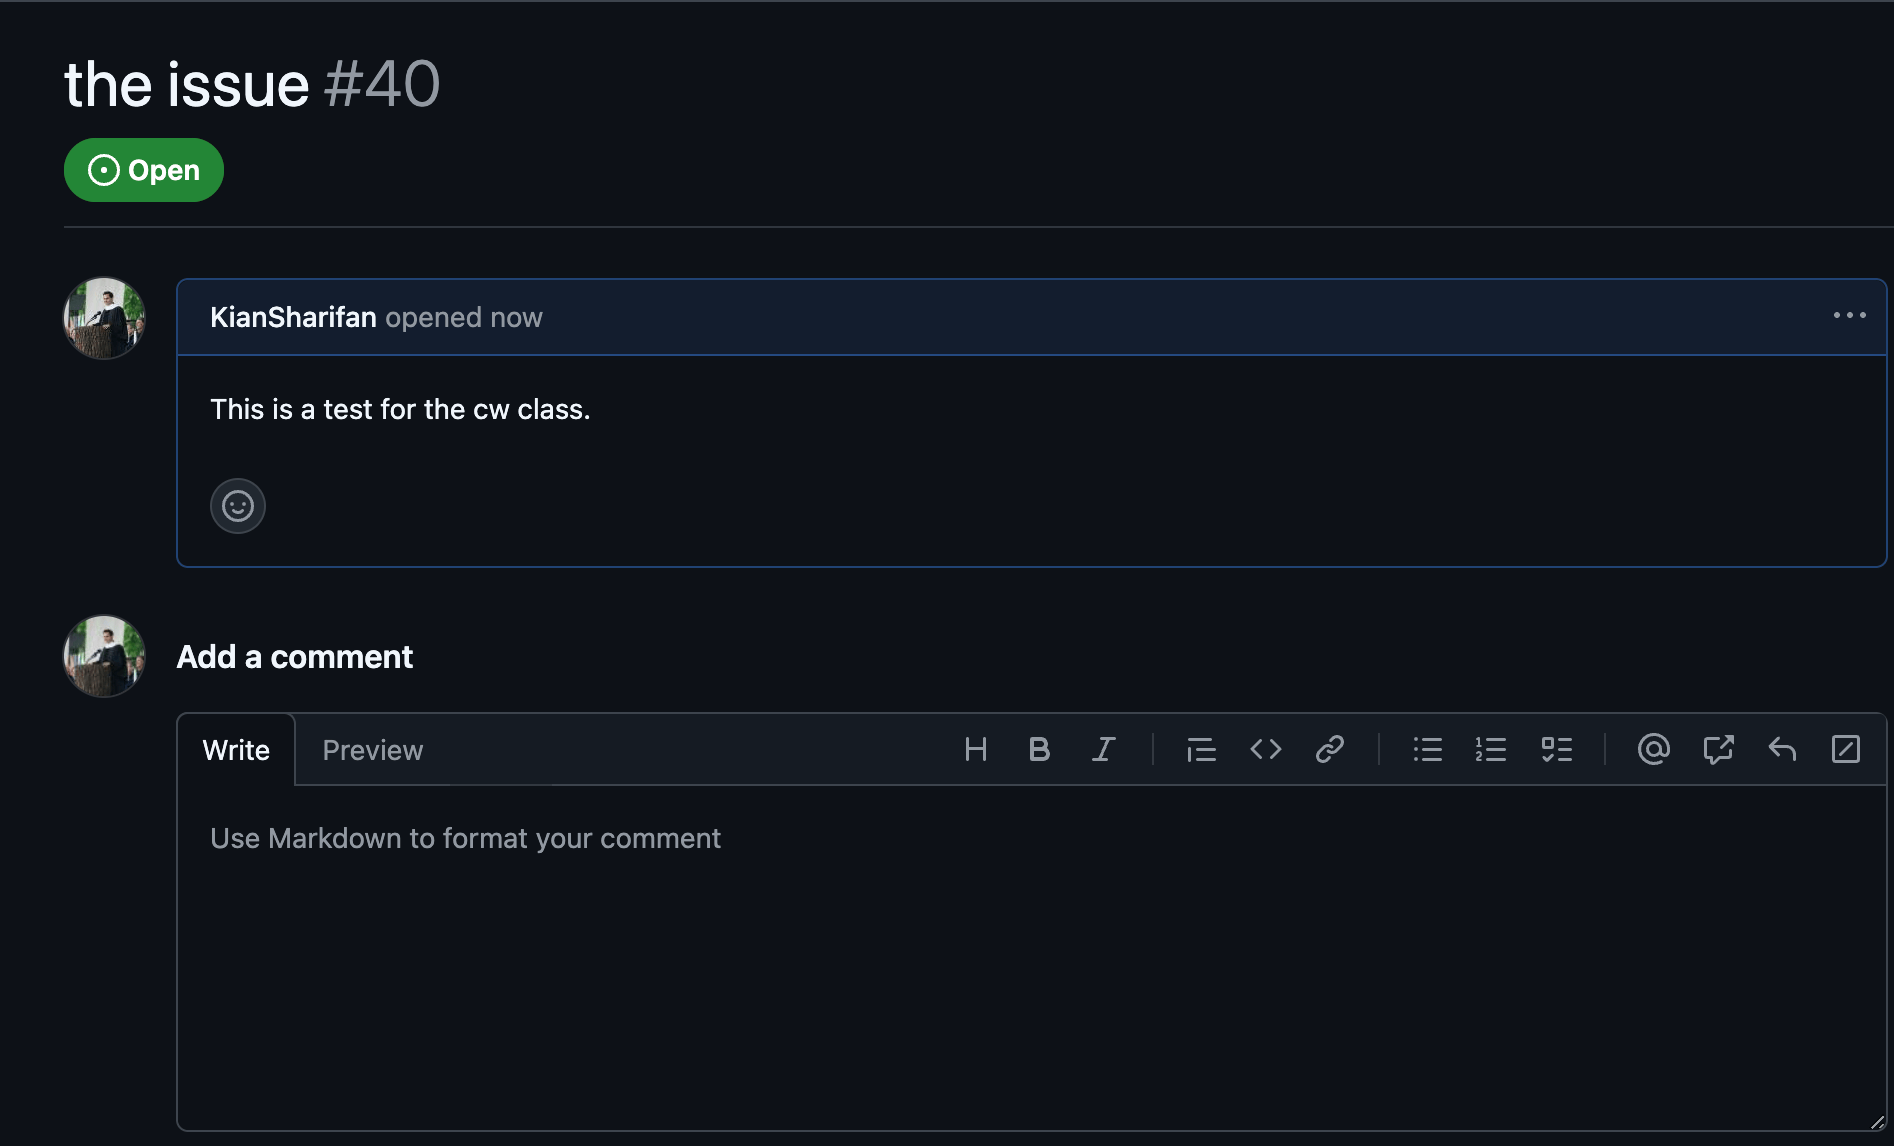
\includegraphics[width=0.75\linewidth]{pic.png}
    \caption{the issue}
    \label{fig:enter-label}
\end{figure}
\subsection{FOSS contribution}
Yes, I can definitely see myself contributing to Free and Open Source Software (FOSS) projects in the future.where i want to contribute : Artificial Intelligence and Natural Language Processing (NLP)
\newline
\newline
The link to the repository:\newline
\large{https://github.com/KianSharifan/cw-final-project}


\end{document}
